%%%%%%%%%%%%%%%%%%%%%%%%%%%%%%%%%%%%%%%%%
% Masters/Doctoral Thesis 
% LaTeX Template
% Version 2.5 (27/8/17)
%
% This template was downloaded from:
% http://www.LaTeXTemplates.com
%
% Version 2.x major modifications by:
% Vel (vel@latextemplates.com)
%
% This template is based on a template by:
% Steve Gunn (http://users.ecs.soton.ac.uk/srg/softwaretools/document/templates/)
% Sunil Patel (http://www.sunilpatel.co.uk/thesis-template/)
%
% Template license:
% CC BY-NC-SA 3.0 (http://creativecommons.org/licenses/by-nc-sa/3.0/)
%
%%%%%%%%%%%%%%%%%%%%%%%%%%%%%%%%%%%%%%%%%

%----------------------------------------------------------------------------------------
%	PACKAGES AND OTHER DOCUMENT CONFIGURATIONS
%----------------------------------------------------------------------------------------

\documentclass[
11pt, % The default document font size, options: 10pt, 11pt, 12pt
%oneside, % Two side (alternating margins) for binding by default, uncomment to switch to one side
english, % ngerman for German
singlespacing, % Single line spacing, alternatives: onehalfspacing or doublespacing
%draft, % Uncomment to enable draft mode (no pictures, no links, overfull hboxes indicated)
%nolistspacing, % If the document is onehalfspacing or doublespacing, uncomment this to set spacing in lists to single
%liststotoc, % Uncomment to add the list of figures/tables/etc to the table of contents
%toctotoc, % Uncomment to add the main table of contents to the table of contents
%parskip, % Uncomment to add space between paragraphs
%nohyperref, % Uncomment to not load the hyperref package
headsepline, % Uncomment to get a line under the header
%chapterinoneline, % Uncomment to place the chapter title next to the number on one line
%consistentlayout, % Uncomment to change the layout of the declaration, abstract and acknowledgements pages to match the default layout
]{MastersDoctoralThesis} % The class file specifying the document structure

\usepackage[utf8]{inputenc} % Required for inputting international characters
\usepackage[T1]{fontenc} % Output font encoding for international characters

\usepackage{mathpazo} % Use the Palatino font by default

\usepackage[backend=bibtex,style=authoryear,natbib=true]{biblatex} % Use the bibtex backend with the authoryear citation style (which resembles APA)

\addbibresource{example.bib} % The filename of the bibliography

\usepackage[autostyle=true]{csquotes} % Required to generate language-dependent quotes in the bibliography

\usepackage{float} %fixar imagens e tabelas
\usepackage{amsmath}
\usepackage{multirow}

%----------------------------------------------------------------------------------------
%	MARGIN SETTINGS
%----------------------------------------------------------------------------------------

\geometry{
	paper=a4paper, % Change to letterpaper for US letter
	inner=2.5cm, % Inner margin
	outer=3.8cm, % Outer margin
	bindingoffset=.5cm, % Binding offset
	top=1.5cm, % Top margin
	bottom=1.5cm, % Bottom margin
	%showframe, % Uncomment to show how the type block is set on the page
}

%----------------------------------------------------------------------------------------
%	THESIS INFORMATION
%----------------------------------------------------------------------------------------

\thesistitle{Dicionário de Machine Learning} % Your thesis title, this is used in the title and abstract, print it elsewhere with \ttitle
\supervisor{Dr. James \textsc{Smith}} % Your supervisor's name, this is used in the title page, print it elsewhere with \supname
\examiner{} % Your examiner's name, this is not currently used anywhere in the template, print it elsewhere with \examname
\degree{Doctor of Philosophy} % Your degree name, this is used in the title page and abstract, print it elsewhere with \degreename
\author{Marcos Augusto \textsc{Barbosa}} % Your name, this is used in the title page and abstract, print it elsewhere with \authorname
\addresses{} % Your address, this is not currently used anywhere in the template, print it elsewhere with \addressname

\subject{Biological Sciences} % Your subject area, this is not currently used anywhere in the template, print it elsewhere with \subjectname
\keywords{} % Keywords for your thesis, this is not currently used anywhere in the template, print it elsewhere with \keywordnames
\university{\href{http://www.university.com}{University Name}} % Your university's name and URL, this is used in the title page and abstract, print it elsewhere with \univname
\department{\href{http://department.university.com}{Department or School Name}} % Your department's name and URL, this is used in the title page and abstract, print it elsewhere with \deptname
\group{\href{http://researchgroup.university.com}{Research Group Name}} % Your research group's name and URL, this is used in the title page, print it elsewhere with \groupname
\faculty{\href{http://faculty.university.com}{Faculty Name}} % Your faculty's name and URL, this is used in the title page and abstract, print it elsewhere with \facname

\AtBeginDocument{
\hypersetup{pdftitle=\ttitle} % Set the PDF's title to your title
\hypersetup{pdfauthor=\authorname} % Set the PDF's author to your name
\hypersetup{pdfkeywords=\keywordnames} % Set the PDF's keywords to your keywords
}

\begin{document}

\frontmatter % Use roman page numbering style (i, ii, iii, iv...) for the pre-content pages

\pagestyle{plain} % Default to the plain heading style until the thesis style is called for the body content

%----------------------------------------------------------------------------------------
%	TITLE PAGE
%----------------------------------------------------------------------------------------

\begin{titlepage}
\begin{center}

\vspace*{.06\textheight}
{\scshape\LARGE \univname\par}\vspace{1.5cm} % University name
\textsc{\Large Doctoral Thesis}\\[0.5cm] % Thesis type

\HRule \\[0.4cm] % Horizontal line
{\huge \bfseries \ttitle\par}\vspace{0.4cm} % Thesis title
\HRule \\[1.5cm] % Horizontal line
 
\begin{minipage}[t]{0.4\textwidth}
\begin{flushleft} \large
\emph{Author:}\\
\href{http://www.johnsmith.com}{\authorname} % Author name - remove the \href bracket to remove the link
\end{flushleft}
\end{minipage}
\begin{minipage}[t]{0.4\textwidth}
\begin{flushright} \large
\emph{Supervisor:} \\
\href{http://www.jamessmith.com}{\supname} % Supervisor name - remove the \href bracket to remove the link  
\end{flushright}
\end{minipage}\\[3cm]
 
\vfill

\large \textit{A thesis submitted in fulfillment of the requirements\\ for the degree of \degreename}\\[0.3cm] % University requirement text
\textit{in the}\\[0.4cm]
\groupname\\\deptname\\[2cm] % Research group name and department name
 
\vfill

{\large \today}\\[4cm] % Date
%\includegraphics{Logo} % University/department logo - uncomment to place it
 
\vfill
\end{center}
\end{titlepage}

%----------------------------------------------------------------------------------------
%	DECLARATION PAGE
%----------------------------------------------------------------------------------------

%\begin{declaration}
%\addchaptertocentry{\authorshipname} % Add the declaration to the table of contents
%\noindent I, \authorname, declare that this thesis titled, \enquote{\ttitle} and the work presented in it are my own. I confirm that:

%\begin{itemize} 
%\item This work was done wholly or mainly while in candidature %for a research degree at this University.
%\item Where any part of this thesis has previously been %submitted for a degree or any other qualification at this %University or any other institution, this has been clearly stated.
%\item Where I have consulted the published work of others, this is always clearly attributed.
%\item Where I have quoted from the work of others, the source is always given. With the exception of such quotations, this thesis is entirely my own work.
%\item I have acknowledged all main sources of help.
%\item Where the thesis is based on work done by myself jointly with others, I have made clear exactly what was done by others and what I have contributed myself.\\
%\end{itemize}
 
%\noindent Signed:\\
%\rule[0.5em]{25em}{0.5pt} % This prints a line for the signature
 
%\noindent Date:\\
%\rule[0.5em]{25em}{0.5pt} % This prints a line to write the %date
%\end{declaration}

\cleardoublepage

%----------------------------------------------------------------------------------------
%	QUOTATION PAGE
%----------------------------------------------------------------------------------------

\vspace*{0.2\textheight}

%\noindent\enquote{\itshape Thanks to my solid academic training, today I can write hundreds of words on virtually any topic without possessing a shred of information, which is how I got a good job in journalism.}\bigbreak

%\hfill Dave Barry

%----------------------------------------------------------------------------------------
%	ABSTRACT PAGE
%----------------------------------------------------------------------------------------

%\begin{abstract}
%\addchaptertocentry{\abstractname} % Add the abstract to the %table of contents
%The Thesis Abstract is written here (and usually kept to just %this page). The page is kept centered vertically so can expand %into the blank space above the title too\ldots
%\end{abstract}

%----------------------------------------------------------------------------------------
%	ACKNOWLEDGEMENTS
%----------------------------------------------------------------------------------------

%\begin{acknowledgements}
%\addchaptertocentry{\acknowledgementname} % Add the %acknowledgements to the table of contents
%The acknowledgments and the people to thank go here, don't %forget to include your project advisor\ldots
%\end{acknowledgements}

%----------------------------------------------------------------------------------------
%	LIST OF CONTENTS/FIGURES/TABLES PAGES
%----------------------------------------------------------------------------------------

\tableofcontents % Prints the main table of contents

%\listoffigures % Prints the list of figures

%\listoftables % Prints the list of tables

%----------------------------------------------------------------------------------------
%	ABBREVIATIONS
%----------------------------------------------------------------------------------------

%\begin{abbreviations}{ll} % Include a list of abbreviations (a table of two columns)

%\textbf{LAH} & \textbf{L}ist \textbf{A}bbreviations \textbf{H}ere\\
%\textbf{WSF} & \textbf{W}hat (it) \textbf{S}tands \textbf{F}or\\

%\end{abbreviations}

%----------------------------------------------------------------------------------------
%	PHYSICAL CONSTANTS/OTHER DEFINITIONS
%----------------------------------------------------------------------------------------

%\begin{constants}{lr@{${}={}$}l} % The list of physical constants is a three column table

% The \SI{}{} command is provided by the siunitx package, see its documentation for instructions on how to use it

%Speed of Light & $c_{0}$ & \SI{2.99792458e8}{\meter\per\second} (exact)\\
%Constant Name & $Symbol$ & $Constant Value$ with units\\

%\end{constants}

%----------------------------------------------------------------------------------------
%	SYMBOLS
%----------------------------------------------------------------------------------------

%\begin{symbols}{lll} % Include a list of Symbols (a three column table)

%$a$ & distance & \si{\meter} \\
%$P$ & power & \si{\watt} (\si{\joule\per\second}) \\
%Symbol & Name & Unit \\

%\addlinespace % Gap to separate the Roman symbols from the Greek

%$\omega$ & angular frequency & \si{\radian} \\

%\end{symbols}

%----------------------------------------------------------------------------------------
%	DEDICATION
%----------------------------------------------------------------------------------------

%\dedicatory{For/Dedicated to/To my\ldots} 

%----------------------------------------------------------------------------------------
%	THESIS CONTENT - CHAPTERS
%----------------------------------------------------------------------------------------

%\mainmatter % Begin numeric (1,2,3...) page numbering

\pagestyle{thesis} % Return the page headers back to the "thesis" style

% Include the chapters of the thesis as separate files from the Chapters folder
% Uncomment the lines as you write the chapters

% Chapter 1

\chapter{Supervised Learning} % Main chapter title

\label{Chapter1} % For referencing the chapter elsewhere, use \ref{Chapter1} 

%----------------------------------------------------------------------------------------

% Define some commands to keep the formatting separated from the content 
\newcommand{\keyword}[1]{\textbf{#1}}
\newcommand{\tabhead}[1]{\textbf{#1}}
\newcommand{\code}[1]{\texttt{#1}}
\newcommand{\file}[1]{\texttt{\bfseries#1}}
\newcommand{\option}[1]{\texttt{\itshape#1}}

%----------------------------------------------------------------------------------------

\section{Initial Considerations}

\begin{enumerate}
    \item Regression: Linear Regression and Generalized Linear Models (GLM's);
    \item Instance-based Algorithms: k-Nearest Neighbor (KNN);
    \item Decision Tree Algorithms: CART (Classification and regression tree);
    \item Bayesian Algorithms: Naive Bayes;
    \item Ensemble Algorithms: Random Forest, AdaBoost, eXtreme Gradient Boosting;
    \item Deep Learning Algorithms: Convolution Neural Network.
\end{enumerate}

%----------------------------------------------------------------------------------------

\section{Linear Regression}
      
    Using the classical linear regression model is justified if we can admit:
    
    \begin{enumerate}
        \item Linearity of the structure of $E(Y)$;
        \item Variance of the error is constant, $Var(Y) = \sigma^2$;
        \item Normality of the observations y's
        \item Independency of the observations y's
    \end{enumerate}
    
    If the assumptions (1) to (3) are not satisfied for the original data, a non-linear transformation of $Y$ might verify them, at least approximately.
    (The Box and Cox models class tries to transform the dependent variable to satisfy the assumptions (1) to (4))
    
    The $R^2$ (Coefficient of Determination) represents the proportion of the total variation explained by the relation of $\textbf{X}$ and $\textbf{Y}$ (regression).
    
    \begin{equation}
        R^2 = \frac{SQReg}{SQT} = 1 - \frac{SQRes}{SQT}
    \end{equation}
    
    Large values of $R^2$ indicates that the total variation of $\textbf{Y}$ is reduced by the insertion of the explanatory variables $X_1, X_2, \dots, X_p$
    Adding more explanatory variables to the model will increase the $R^2$. So, here is the $R^2_{adjusted}$, given by
    
    \begin{equation}
        R^2 = 1 - \frac{SQRes/(n-(p+1))}{SQT/(n-1)}
    \end{equation}
    
    $R^2_{adjusted}$ will increase when the explanatory variable addition reduces the $SQRes/(n-(p+1))$
    

\section{Generalized Linear Models}

Using the generalized linear model is justified if we can admit:
    
\begin{enumerate}
    \item $Y_i$'s are independent;
    \item $Y$ belongs to a exponential family $FE(\theta, \phi)$;
    \item Exists a function g (doubly differentiable and invertible) that relates the $\mu_i$ to a linear predictor $\eta_i = \beta_0 + \beta_1X_{1i} + \beta_2X_{2i}$
\end{enumerate}
    
The linear predictor can return values from $(-\infty, \infty)$. So if the response variable is in that interval, like a normal distribution and the link function is the identity, it is great! But if the response variable is always positive and if the mean is too distant from the zero, you can actually use the classical linear regression, because even though the linear predictor is able to return negative values, the mean is too distant from the zero and there are few values close to zero, it would not probably be able to predict negative values (unless in some extreme combination of covariables values).

\section{Mixture Models for Density Estimation and
Classification}

The mixture model is a useful tool for density estimation, and can be viewed
as a kind of kernel method. The Gaussian mixture model has the form

\begin{equation}
    f(x) = \sum^{M}_{m=1} \alpha_m\phi(x; \mu_m, \boldsymbol{\Sigma}_m)
\end{equation}

with mixing proportions $\alpha_m$, $\Sigma_m\alpha_m = 1$, and each Gaussian density has a mean $\mu_m$ and covariance matrix $\boldsymbol{\Sigma}_m$. In general, mixture models can use any component densities in place of the Gaussian in (6.32): the Gaussian mixture model is by far the most popular.

The parameters are usually fit by maximum likelihood, using the EM
algorithm as described in Chapter 8. 

Posso utilizar esse modelo quando há apenas uma variável em disposição? Sim e para quano tiver mais de uma também 

In the multivariate Gaussian mixture problem (see Exercise 12.9), the
“curse of dimensionality” raises its ugly head, where the number of para-
meters grows quickly with the increase in dimensionality. Although PCA
is often used as a first step to reduce the dimensionality, this does not help in mixtures problems because any class structure as exists may not be pre- served by the principal components (Chang, 1983).

\section{k-nearest neighbours (classifiers)}
These classifiers are memory-based and require no model to be fit. Given a query point $x_0$, we find the $k$ training points $x(r), r = 1, \dots,k$ closest in distance to $x_0$, and then classify using majority vote among the $k$ neighbors. Ties are broken at random. For simplicity we will assume that the features are real-valued, and we use Euclidean distance in feature space:

\begin{equation}
    d(i) = ||x(i) - x_0||
\end{equation}

Typically we first standardize each of the features to have mean zero and variance 1, since it is possible that they are measured in different units.

\section{Support Vector Machines (SVM's)}
Mostly used in classification problems. We may want to enlarge our feature space in order to accommodate a non-linear boundary between the classes. Produces nonlinear boundaries by constructing a linear boundary in
a large, transformed version of the feature space. The kernel approach that we describe here is simply an efficient computational approach for enacting this idea. What is the advantage of using a kernel rather than simply enlarging the feature space using functions of the original features, as in (9.16)? One advantage is computational, and it amounts to the fact that using kernels, one need only compute $K(x_i, x_i^{'})$ for all (n 2) distinct pairs $i, i^{'}$. This can be done without explicitly working in the enlarged feature space.
\begin{itemize}
    \item Advantages: efective tool in high-dimensional spaces, memory efficient (Since only a subset of the training points are used in the
    actual decision process of assigning new members, just these points need
    to be stored in memory and calculated upon when making decisions and versatility (Class separation is often highly non-linear. The ability to apply new kernels allows substantial flexibility for the decision boundaries, leading to greater classification performance)
    \item Disadvantages: SVMs are very sensitive to the choice of the kernel parameters and there is no direct probabilistic interpretation for group membership and the black box nature of these functions. The use of kernels to separate non-linear data makes them difficult (if not impossible) to interpret. Despite its popularity, SVM has a serious drawback, that is sensitivity to outliers in training samples. The penalty on misclassification is defined by a convex loss called the hinge loss, and the unboundedness of the convex loss causes the sensitivity to outliers.
\end{itemize}

\section{Random Forest}

The essential idea in bagging (Section 8.7) is to average many noisy but
approximately unbiased models, and hence reduce the variance. Trees are
ideal candidates for bagging, since they can capture complex interaction
structures in the data, and if grown sufficiently deep, have relatively low
bias. Since trees are notoriously noisy, they benefit greatly from the averaging. Moreover, since each tree generated in bagging is identically distributed (i.d.), the expectation of an average of B such trees is the same as the expectation of any one of them. This means the bias of bagged trees is the same as that of the individual (bootstrap) trees, and the only hope of improvement is through variance reduction. This is in contrast to boosting, where the trees are grown in an adaptive way to remove bias, and hence are not i.d.

The idea in random forests (Algorithm 15.1) is to improve
the variance reduction of bagging by reducing the correlation between the
trees, without increasing the variance too much. This is achieved in the
tree-growing process through random selection of the input variables.

Combination of many decision trees, effectively leveraging and combining the choices of many models (this technique of using a combination of models is known as \textbf{ensembling}).

Para classificação, uma medida de impureza que pode ser usada é:
\begin{itemize}
    \item Misclassification error
    \item Gini index
    \item Cross-entropy or deviance
    
\end{itemize}

Para regressão, uma medida de impureza que pode ser usada é  $SSE = \sum_{i \in S_1} (y_i - \bar(y)1)^2 + \sum_{i \in S_2} (y_i - \bar(y)2)^2$.

Out-of-Bag sample, no contexto de \textit{random forest}, consiste na observação que não foi selecionada na amostra \textit{bootstrap} utilizada por uma determinada árvore de decisão.

Out-of-Bag error, no contexto de \textit{random forest}, consiste na proporção de \textit{out-of-bag samples} incorretamente classificadas.

\section{AdaBoost}
How weights are updated in AdaBoost? Simply put, the idea is to set weights to both classifiers and data points (samples) in a way that forces classifiers to concentrate on observations that are difficult to correctly classify. This process is done sequentially in that the two weights are adjusted at each step as iterations of the algorithm proceed. 

AdaBoost is also extremely sensitive to Noisy data and outliers so if you do plan to use AdaBoost then it is highly recommended to eliminate them. AdaBoost has also been proven to be slower than XGBoost.

\section{Gradient Boosting Machine (Regression)}
We start with a leaf that is the average value of the variable we want to predict. Then we add a tree based on the Residuals, tree is scaled by a contrbution (fixed learning rate). Then we add another tree based on the new residuals and we keep adding trees based on the errors made by the previous tree.

\section{XGBoost}

XGBoost is an exceptionally useful machine learning method when you don't want to sacrifice the ability to correctly classify observations but you still want a model that is fairly easy to understand and interpret. 


XGBoost, scalable machine learning system for tree boosting, was designed to be used with large, complicated datasets. Just like Gradient Boost (unextreme), XGBost fits a Regression Tree to the residuals but uses a unique Regression Tree. Let's callt it XGBoost tree.

We prune the XGBoost tree based on the gain of the branch and a $\gamma$

$\lambda$ is a regularization parameter, which means that it is intended to reduce the prediction's sensitivity to individual observations, prevents over fitting the training data. It results in more pruning, by shrinking the Similarity Scores and it results in smaller Output Values for the leaves

There is a learning rate parameter also.

We calculate Similarity Scores and Gain to determine how to split the data and we prune the tree by calculating the differences between Gain values and a user defined Tree Complexity Parameter $\gamma$. If positive, then do not prune. If negative, then prune.

Then we calculate the Output Values for the remaining leaves.

The minimum number of Residuals in each leaf is determined by calculating something called Cover

One thing that is relatively unique about XGBoost is that it has default behavior for missing data. In Python, all we have to do is identify missing values and make sure they are set to 0

Uses the Second Order Taylor Approximation for both Regression and Classification.

For classification, the negative log-likelihood is the most commonly used loss function.

There are several different ways to calculate feature importances. By default, “gain” is used, that is the average gain of the feature when it is used in trees. Other types are “weight” - the number of times a feature is used to split the data, and “cover” - the average coverage of the feature. You can pass it with $importance_type$ argument.

%----------------------------------------------------------------------------------------

\section{Neural Networks}

\begin{figure}[H]
\centering
\caption{NeuralNetwork}
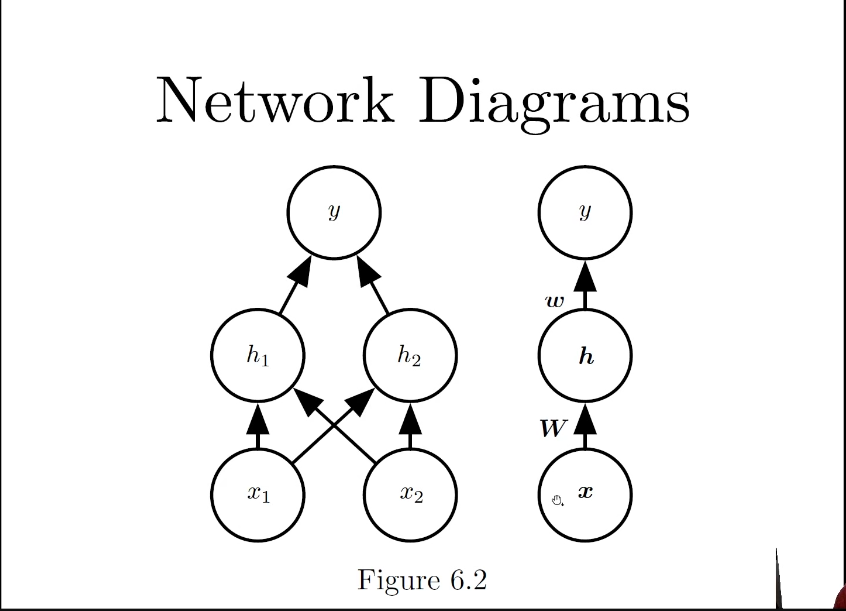
\includegraphics[scale=0.5]{Figures/network-diagram.PNG}
\end{figure}

Back-propagation is "just the chain rule" of calculus, one of the key concepts of NN. É um algortimo para calcular o gradiente de modo extramammente eficiente (baixa complexidade computacional), Is the method to calculate the gradient of the loss function with respect to the weights in an artificial neural network

\begin{enumerate}
    \item Forward prop: start an the input x, apply the weight and biases and compute y and the cost
    \item Back prop: based on the  associated y and cost, update weighs and biases?
    \item
\end{enumerate}

When we use a feedforward neural network to accept an input $\boldsymbol{x}$ and produce an
output $\hat{\boldsymbol{y}}$, information flows forward through the network. The inputs x provide
the initial information that then propagates up to the hidden units at each layer
and finally produces $\hat{\boldsymbol{y}}$ . This is called forward propagation . During training,
forward propagation can continue onward until it produces a scalar cost $J (\boldsymbol{\theta})$.
The back-propagation algorithm,  often simply called backprop, allows the information from the cost to then flow backwards through
the network, in order to compute the gradient.


The term back-propagation is often misunderstood as meaning the whole
learning algorithm for multi-layer neural networks. Actually, back-propagation refers only to the method for computing the gradient

Activating functions: the softmax function is used as the activation function in the output layer of neural network models that predict a multinomial probability distribution. That is, softmax is used as the activation function for multi-class classification problems where class membership is required on more than two class labels.

\section{Time Series Models}
Para verificar o poder preditivo do modelo é interessante comparar as métricas de performance do modelo proposto com as de um \textit{naive forecast model} (benchmarking)

\subsection{ARMA}
Modelos ARMA só podem ser aplicados para séries estacionárias. No
entanto, a maior parte das séries não são estacionárias.
\subsection{ARIMA}
Um modelo ARMA Integrado, ARIMA(p,d,q), consiste em aplicar o
modelo ARMA(p,q) na d-ésima diferença da série. Aplicar d-diferenças torna a série estacionária. Geralmente d = 1 ou d = 2 é suficiente para séries não sazonais (ou com sazonalidade ajustada)
\subsection{SARIMA}
\subsection{ARIMAX}
\subsection{SARIMAX}

\section{Conceitos importantes}

\subsection{Multicolinearidade}
Multicollinearity happens when independent variables in the regression model are highly correlated to each other. It makes it hard to interpret of model and also creates an overfitting problem. It is a common assumption that people test before selecting the variables into the regression model. How to check wheter Multicollinearity occurs?

\begin{enumerate}
    \item Plot the correlation matrix of all the independent variables
    \item Use the Variance Inflation Factor (VIF) for each independent variable. It is a measure of multicollinearity in the set of multiple regression variables. The higher the value of VIF the higher correlation between this variable and the rest.
\end{enumerate}

How to fix the Multi-Collinearity issue?
\begin{enumerate}
    \item Variable selection
    \item Variable transformation
    \item PCA (Principal Component Analysis): the character of variable independence
\end{enumerate}

\subsection{Cross Validation}
Consiste em dividir o conjunto de dados (treino + teste) em $k$ pedaços. Em seguida, para cada combinação de $k-1$ pedaços, é ajustado o modelo de interesse e calculado, no pedaço restante, a(s) métrica(s) de validação. Útil para comparar a performance entre modelos distintos e para selecionar os melhores  \textit{tunning parameters}. Algumas variações desse procedimento:

\begin{enumerate}
    \item \textbf{K-Fold Cross Validation}
    \item \textbf{Leave One Out Cross Validation}
    \item  \textbf{Repeated Cross Validation}
\end{enumerate}

\subsection{Bagging (Boostrap Aggregating)}
Dado um conjunto de dados de treino, o procedimento \textit{bagging} gera novas $m$ amostras com reposição desse conjunto (esse tipo de amostra é chamada de \textit{bootstrap}), para, em seguida, ajustar $m$ modelos nas $m$ amostras \textit{bootstrap} (um modelo para cada amostra) e combinar o output em uma média (no caso de regressão) ou votação (no caso de classificação). The essential idea in bagging is to average many noisy but approximately unbiased models, and hence reduce the variance. The number of trees B is not a critical parameter with bagging; using a very large value of B will not lead to overfitting. In practice we use a value of B sufficiently large that the error has settled down.

\begin{figure}[H]
\centering
\caption{Illustration of bagging}
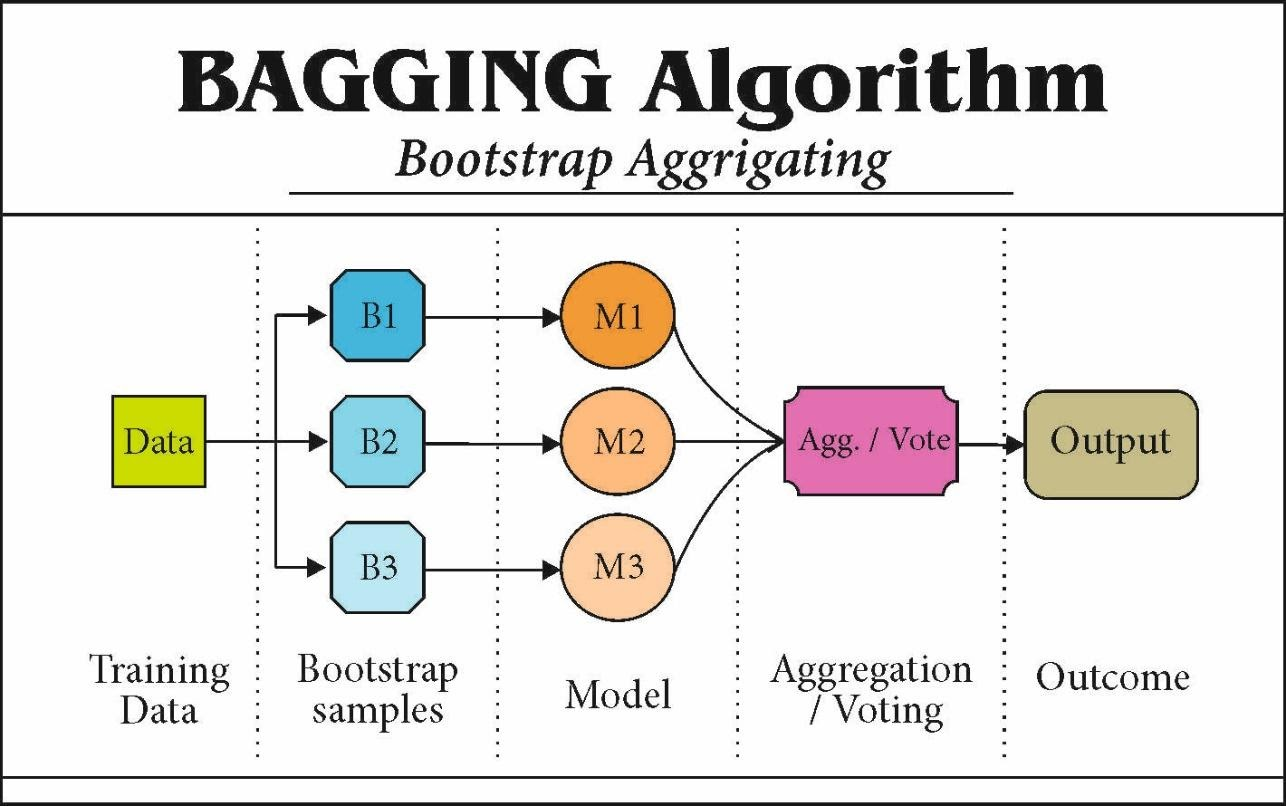
\includegraphics[scale=0.2]{Figures/bagging.jpg}
\end{figure}


\subsection{Boosting}
A weak classifier is one whose error rate is only slightly better than
random guessing. The purpose of boosting is to sequentially apply the
weak classification algorithm to repeatedly modified versions of the data,
thereby producing a sequence of weak classifiers $G_m(x)$, $m = 1, 2,\dots, M$.

Boosting works in a similar way of the bagging procedure except that the trees are grown sequentially: each tree is grown using information from previously grown trees. Boosting does not involve bootstrap sampling; instead each tree is fit on a modified version of the original data set. Boosting has three parameters:

\begin{enumerate}
    \item The number of trees B. Unlike bagging and random forests, boosting can overfit if B is too large, although this overfitting tends to occur slowly if at all. We use cross-validation to select B.
    
    \item The shrinkage parameter $\lambda$, a small positive number. This controls the rate at which boosting learns. Typical values are 0.01 or 0.001, and the right choice can depend on the problem. Very small $\lambda$ can require using a very large value of B in order to achieve good performance.
    
    \item The number $d$ of splits in each tree, which controls the complexity of the boosted ensemble. Often $d$ = 1 works well, in which case each tree is a stump, consisting of a single split. In this case, the boosted ensemble is fitting an additive model, since each term involves only a single variable. More generally $d$ is the interaction depth, and controls the interaction order of the boosted model, since $d$ splits can involve at most $d$ variables.
\end{enumerate}

\subsection{Regularization}
Regularized regression consists in estimating a penalized function of the form.

\begin{equation}
\underset{f \in H}{min} \Big[ \sum_{i = 1}^{N}
L(y_i, f(x_i)) + \lambda J(f) \Big ], 
\end{equation},

where $L(y, f(x))$ is the chosen loss function, $J(f)$ is a penalty functional and $H$ is a space of function on which $J(f)$ is defined (Hastie, Tibshirani, and Friedman, 2009)

Produces models that are more parsimonious and have similar prediction error as the full model and it is usually robust enough to not be influenced by the correlated variables. 
    
For tree-based methods, there is not yet a well established regularization procedure in the literature.

\begin{enumerate}
\item \textbf{Ridge Regression (L2)}: consiste em adicionar uma penalidade equivalente aos quadrados das magnitudes dos coeficientes, na função de custo. É útil para fazer \textit{shrink} das estimativas dos parâmetros (pode chegar perto de zero, mas não exatamente 0) e reduzir a complexidade do modelo e a multicolinearidade. Conforme \textit{Introduction to Statistical Learning}, tem-se que \textit{it is best to apply ridge regression after standardizing the predictors}.

When the number of variables $p$ is almost as large as the number of observtions $n$, the OLS estimates will be extremely variable. And if $p > n$, then the OLS estimates do not even have a unique solution, whereas ridge regression can still perform well by trading off a small increse in bias for a large decrease in variance (bias and variance tradeoff)

\item \textbf{Lasso  Regression (L1)}: consiste em adicionar uma penalidade equivalente às magnitudes dos coeficientes, na função de custo. É útil para reduzir \textit{overfitting} e selecão de variáveis (os coeficientes podem chegar a zero). Sendo assim, resulta em uma equação mais imples e mais fácil de interpretar.

\item \textbf{Regularization Elastic Net}: consiste em uma combinação entre \textit{Ridge Regression (L1)} e \textit{Lasso Regression (L2)}. Pode ajudar a excluir certos parâmetros.
\end{enumerate}

\subsection{Métricas de avaliação}
\subsubsection{Regressão}

\begin{enumerate}
    \item Mean Squared Error (MSE):
    
    \begin{equation}
        MSE = \frac{1}{n}\sum^n_{i=1}(Y_i - \hat{Y}_i)^2
    \end{equation}
    
    Like variance, mean squared error has the disadvantage of heavily weighting outliers.[11] This is a result of the squaring of each term, which effectively weights large errors more heavily than small ones. This property, undesirable in many applications, has led researchers to use alternatives such as the mean absolute error, or those based on the median. 
    \item Mean Absolute Error (MAE)
    \item Mean Absolute Percentage Error (MAPE)
\end{enumerate}

\subsubsection{Classificação}

\begin{table}[H]
\centering
\caption{Matriz de Confusão}
\begin{tabular}{@{}cc cc@{}}
\multicolumn{1}{c}{} &\multicolumn{1}{c}{} &\multicolumn{2}{c}{\textbf{Predição}} \\ 
\cmidrule(lr){3-4}
\multicolumn{1}{c}{} & 
\multicolumn{1}{c}{} & 
\multicolumn{1}{c}{False (-)} & 
\multicolumn{1}{c}{True (+)} \\ 
\cline{2-4}
\multirow[c]{2}{*}{\rotatebox[origin=tr]{0}{\textbf{Classe}}}
& False (-) & TN (True Negative) & FP (False Positive) \\[1.5ex]
& True (+) & FN (False Negative)   & TP (True Positive) \\
\cline{2-4}
\end{tabular}
\label{confusion-matrix}
\end{table}

\begin{align*}
\text{Accuracy} &= \frac{TN + TP}{TN + FP + FN + TP}\\
\text{Precision} &= \frac{TP}{TP + FP}\\
\text{Recall, Sensitivity, True Positive Rate} &= \frac{TP}{TP + FN}\\
\text{F1 Score} &= 2\frac{precision * recall}{precision + recall}\\
\end{align*}

É interessante fazer a Curva ROC, gráfico entre \textit{True Positive Rate} e \textit{False Positive Rate} (FP / (FP + TN)). It summarizes all of the confusion matrices that each threshold produced.

A utilização da acurácia não é recomendado no caso de um conjunto de dados desbalanceados.


% Chapter Template

\chapter{Unsupervised Learning} % Main chapter title

\label{Chapter2} % Change X to a consecutive number; for referencing this chapter elsewhere, use \ref{ChapterX}

%----------------------------------------------------------------------------------------
%	SECTION 1
%----------------------------------------------------------------------------------------

\section{Partitioning Methods}

Suitable for finding spherical-shaped clusters or convex clusters. In other words, they work well for compact and well separated clusters. Moreover, they are also severely affected by the presence of noise and outliers in the data. Unfortunately, real life data can contain: i) clusters of arbitrary shape (oval, linear and “S” shape clusters); ii) many outliers and noise.
\subsection{K-means}
There are various methods to find the optimal/best value of k. In this article we will cover two:

\begin{itemize}
\item Elbow Method

\item Silhouette Method: The silhouette Method is also a method to find the optimal number of clusters and interpretation and validation of consistency within clusters of data. The silhouette method computes silhouette coefficients of each point that measure how much a point is similar to its own cluster compared to other clusters by providing a succinct graphical representation of how well each object has been classified. Compute silhouette coefficients for each of point, and average it out for all the samples to get the silhouette score

The value of the silhouette ranges between [1, -1], where a high value indicates that the object is well matched to its own cluster and poorly matched to neighboring clusters.
    
\end{itemize}

Importante pensar cuidadosamente se é necessário padronizar as variáveis (deixá-las com desvio-padrão igual 1).
    
\subsection{PAM clustering}
\subsection{Clusterização Hierárquica}

É importante pensar cuidadosamente se é necessário padronizar as variáveis (deixá-las com desvio-padrão igual 1). alguns métodos de aglomeração:
\begin{itemize}

\item \textit{Single-Linkage}: mínima dissimilaridade intercluster. Consiste em em computar todas as \textit{pairwise} dissimilaridades entre as observações do cluster A e as observações do cluster B e registrar a menor dessas dissimilaridades.

\item \textit{Complete-Linkage}: máxima dissimilaridade intercluster. Consiste em em computar todas as \textit{pairwise} dissimilaridades entre as observações do cluster A e as observações do cluster B e registrar a maior dessas dissimilaridades. Tende a gerar cluster's mais balanceados.

\item \textit{Average-Linkage}: média dissimilaridade intercluster. Consiste em em computar todas as \textit{pairwise} dissimilaridades entre as observações do cluster A e as observações do cluster B e registrar a média dessas dissimilaridades.
Tende a gerar cluster's mais balanceados.

\item \textit{Centroid-Linkage}: dissimilaridade entre centróide do cluster A e centróide do cluster B. Pode resultar em indesejáveis inversões.

\end{itemize}

\section{Density methods}
\subsection{DBScan (Density-Based Spatial Clustering and Application with Noise)} Non-linear algorithm and it is insensitive to order. Unlike to K-means, DBSCAN does not require the user to specify the number of clusters to be generated, DBSCAN can find any shape of clusters. The cluster doesn’t have to be circular. DBSCAN can identify outliers.

%----------------------------------------------------------------------------------------
%	SECTION 2
%----------------------------------------------------------------------------------------

\section{Considerações}
\begin{itemize}
\item Should the observations or features first be standardized in some way? For instance, maybe the variables should be centered to have mean zero and scaled to have standard deviation one.

\item In the case of hierarchical clustering,

\begin{enumerate}
    \item What dissimilarity measure should be used? Euclidiana, alguma distância baseada em correlação?
    
    \item What type of linkage should be used?
    
    \item Where should we cut the dendrogram in order to obtain clusters?
\end{enumerate}

\item In the case of K-means clustering, how many clusters should we look for in the data?
\end{itemize} 
% Chapter Template

\chapter{Implementação de modelo ML} % Main chapter title

\label{ChapterX} % Change X to a consecutive number; for referencing this chapter elsewhere, use \ref{ChapterX}

%----------------------------------------------------------------------------------------
%	SECTION 1
%----------------------------------------------------------------------------------------

\section{Considerações Iniciais}

Conforme Vincent, o foco deve estar em entender com profundidade o problema, dar um passo atrás e ser humilde, se para você, o problema ainda não está claro. Não se deve focar, em primeiro lugar na solução, e pensar o problema como algo meramente analítico ("Vou ajustar uma rede neural e encontrar os melhores hiperparâmetros e o problema será resolvido!). De modo geral, o que mas importa é todo o conjunto de componentes ao redor do modelo de ML, não o modelo em si. As componentes seriam:

\begin{itemize}
\item Quais dados temos acesso?
\item Qual é a utilidade do modelo para o usuário final?
\item Como seria feito o monitoramento do modelo? Quão complicado seria corrigir erros podem surgir em produção? Corrigir erros de uma regressão linear é muito mais fácil e rápido que corrigir os erros de uma rede neural com milhares/milhões de parâmetros
\item Um sistema simples de regras poderia desempenhar tão bem quanto um modelo de ML?
\item Como avaliar a qualidade do modelo proposto? Há algum benchmark? Pode-se criar um benchmark?
\item Fazer um desenho à mão de toda a arquitetura é uma boa ideia
\end{itemize}

%-----------------------------------
%	SUBSECTION 1
%-----------------------------------
\section{Particionamento dos Dados}
\begin{figure}[H]
\centering
\caption{Data Partitioning}
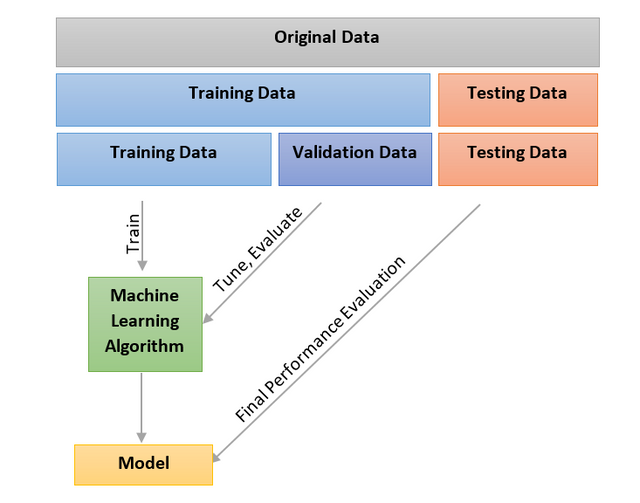
\includegraphics[scale=1.0]{validation.png}
\end{figure}

\begin{itemize}
\item We usually devide the data to train and test set. We will not touch test set until the end of the computation and the final perpormance evaluation. Then, we can devide the train set to train and validation sets. We use the validation data set to tune the model.
\item Traditional train test method suffer from high variance test problem. It means tha by changing the test set the result of the prediction changes. To over come this problem we use k-fold validation method in our train and validation set

\item Separating samples into training and test sets is not always enough. There can be various reasons for duplicate samples that appear in both sets, and it is important to detect and remove these duplicates. For example, one of the most used datasets in Computer Vision, CIFAR, is shown to contain duplicate samples in training and test sets. This becomes more of a problem for models that are trained on huge amounts of data such as BERT and GPT-3. Best practices: Remove duplicates before splitting the data, check for partial duplicates as well, sort by different columns, and examine the data.

\end{itemize}    

%-----------------------------------
%	SUBSECTION 2
%-----------------------------------

\section{Passo a Passo}

\begin{enumerate}
\item Estudo profundo das fontes de informação disponíveis (banco de dados, API's, planilhas);

\item Identificação de variáveis relevantes. Essa etapa costuma assumir um dos dois caminhos seguintes:
\begin{enumerate}
    \item Um seleção de variáveis é feita, com base no conhecimento do negócio envolvido. Se o cientista de dados não conhece bem o campo de conhecimento envolvido, fica difícil fazer isso. Então, consultar especialistas é extremamente recomendado
    
    \item Milhões, milhares de variáveis são escolhidas e jogadas para treinar o modelo mais para frente.
\end{enumerate}

\item Fazer Exploratory Data Analysis do conjunto de dados:

\begin{itemize}
    \item Há dados faltantes?
    \item Há dados que não fazem sentido algum? Por exemplo, uma pessoa tem altura negativa!
    \item As strings, para uma determinada coluna, são consistentes? Por exemplo, a string que se refere a cidade "New York" possui diferentes formatos, e.g., "NEWYORK", "ny", "NY", "new york".
    
\end{itemize}

\section{Considerações sobre predição}
Um modelo de aprendizado de máquina supervisionado treinado com um conjunto de dados de treino é capaz de fazer predições e, por meio dele, conseguimos testar sua performance no conjunto de dados de teste.

Contudo, é de extrema importância que um modelo de ML, em produção, em uma empresa ou aplicação na vida real passe por uma análise de sua performance com um conjunto de dados que só será obtido no futuro. 

Um modelo que classifica se uma reserva de hotel será cancelada, com o snapshot dos dados atuais "apenas" classifica as observações em não canceladas ou canceladas. Entretanto, a gerência do hotel (usuário do modelo) está interessada especificamente em prever, no futuro, um cancelamento. Classificar uma observação atual em não cancelada ou cancelada é algo distinto de prever, no futuro, um cancelamento de reserva de hotel.

Sendo assim, é necessário que de tempos em tempos, com novas safras de dados e as previsões feitas antecipadamente sejam estudadas. É necessário simular o uso final do modelo! 

\end{enumerate}
% Chapter Template

\chapter{Outros tópicos de ML} % Main chapter title

\label{ChapterX} % Change X to a consecutive number; for referencing this chapter elsewhere, use \ref{ChapterX}

%----------------------------------------------------------------------------------------
%	SECTION 1
%----------------------------------------------------------------------------------------

\section{“Off-the-Shelf” Procedures for Data Mining}
Predictive learning is an important aspect of data mining. As can be seen
from this book, a wide variety of methods have been developed for predic-
tive learning from data. For each particular method there are situations
for which it is particularly well suited, and others where it performs badly
compared to the best that can be done with that data. We have attempted
to characterize appropriate situations in our discussions of each of the re-
spective methods. However, it is seldom known in advance which procedure
will perform best or even well for any given problem. Table 10.1 summarizes
some of the characteristics of a number of learning methods.
Industrial and commercial data mining applications tend to be especially
challenging in terms of the requirements placed on learning procedures.
Data sets are often very large in terms of number of observations and
number of variables measured on each of them. Thus, computational considerations play an important role. Also, the data are usually messy: the
inputs tend to be mixtures of quantitative, binary, and categorical vari-
ables, the latter often with many levels. There are generally many missing
values, complete observations being rare. Distributions of numeric predic-
tor and response variables are often long-tailed and highly skewed. This
is the case for the spam data (Section 9.1.2); when fitting a generalized
additive model, we first log-transformed each of the predictors in order to
get a reasonable fit. In addition they usually contain a substantial fraction
of gross mis-measurements (outliers). The predictor variables are generally
measured on very different scales.
In data mining applications, usually only a small fraction of the large
number of predictor variables that have been included in the analysis are
actually relevant to prediction. Also, unlike many applications such as pat-
tern recognition, there is seldom reliable domain knowledge to help create
especially relevant features and/or filter out the irrelevant ones, the inclu-
sion of which dramatically degrades the performance of many methods.
In addition, data mining applications generally require interpretable mod-
els. It is not enough to simply produce predictions. It is also desirable to
have information providing qualitative understanding of the relationship
between joint values of the input variables and the resulting predicted re-
sponse value. Thus, black box methods such as neural networks, which can
be quite useful in purely predictive settings such as pattern recognition,
are far less useful for data mining.
These requirements of speed, interpretability and the messy nature of
the data sharply limit the usefulness of most learning procedures as off-
the-shelf methods for data mining. An “off-the-shelf” method is one that
can be directly applied to the data without requiring a great deal of time-
consuming data preprocessing or careful tuning of the learning procedure.
Of all the well-known learning methods, decision trees come closest to
meeting the requirements for serving as an off-the-shelf procedure for data
mining. They are relatively fast to construct and they produce interpretable
models (if the trees are small). As discussed in Section 9.2, they naturally
incorporate mixtures of numeric and categorical predictor variables and
missing values. They are invariant under (strictly monotone) transforma-
tions of the individual predictors. As a result, scaling and/or more general
transformations are not an issue, and they are immune to the effects of pre-
dictor outliers. They perform internal feature selection as an integral part
of the procedure. They are thereby resistant, if not completely immune,
to the inclusion of many irrelevant predictor variables. These properties of
decision trees are largely the reason that they have emerged as the most
popular learning method for data mining.
Trees have one aspect that prevents them from being the ideal tool for
predictive learning, namely inaccuracy. They seldom provide predictive ac-
curacy comparable to the best that can be achieved with the data at hand.
As seen in Section 10.1, boosting decision trees improves their accuracy,
often dramatically. At the same time it maintains most of their desirable
properties for data mining. Some advantages of trees that are sacrificed by
boosting are speed, interpretability, and, for AdaBoost, robustness against
overlapping class distributions and especially mislabeling of the training
data. A gradient boosted model (GBM) is a generalization of tree boosting
that attempts to mitigate these problems, so as to produce an accurate and
effective off-the-shelf procedure for data mining.

\begin{figure}[H]
\centering
\caption{LearningMethods}
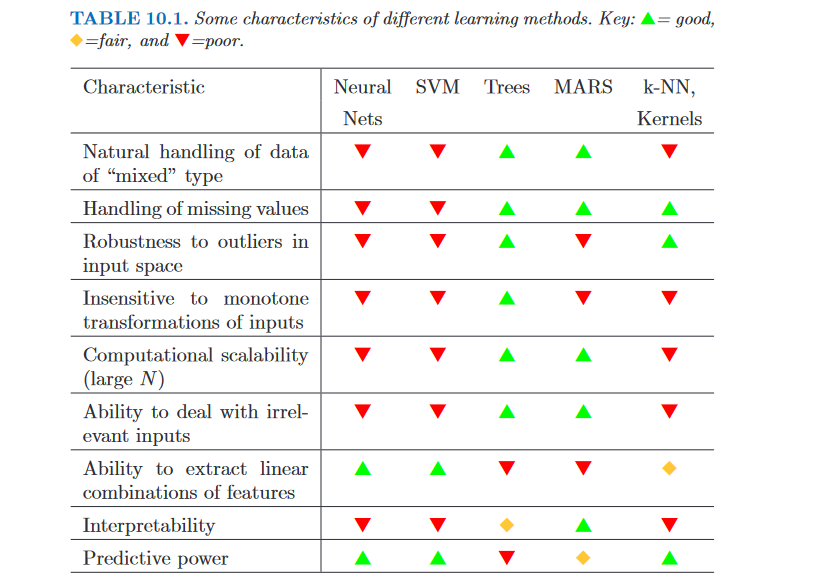
\includegraphics[scale=.7]{Figures/learning-methods.PNG}
\end{figure}

\section{Principal Components Analysis}
The basic goal of principal components analysis is to describe variation in a set of correlated variables, $\textbf{x}^T = (x_1, \dots, x_q)$ in terms of new set of uncorrelated variables $\textbf{y}^T = (y_1, \dots, y_q)$, each of which is a linear combination of the $\textbf{x}$ variables.

The new variables are derived in decreasing order of “impor-
tance” in the sense that $y_1$ accounts for as much as possible of the variation in
the original data amongst all linear combinations of $\textbf{x}$. Then $y_2$ is chosen to
account for as much as possible of the remaining variation, subject to being
uncorrelated with $y_1$, and so on. The new variables defined by this process,
$y_1, \dots, y_q$ , are the principal components.

The first principal component of the observations, y1, is the linear combination

\begin{equation}
    y_1 = a_{11}x_1 + a_{12}x_2 + \dots + a_{1q}x_q
\end{equation}

whose sample variance is greatest among all such linear combinations. Because the variance of $y_1$ could be increased without limit simply by increasing the coefficients $a_1^T = (a_{11}, a_{12}, \dots, a_{1q}x_q)$, a restriction must be placed on these coefficients. To find the coefficients defining the first principal component, we need to choose the elements of the vector  $\textbf{a}_1$
so as to maximize the variance of $y_1$ subject to the sum of squares constraint, which can be written $\textbf{a}_1^T\textbf{a}_1 = 1$. The sample variance of $y_1$ that is a linear function of the $x$ variables is given by $\textbf{a}_1^T\textbf{S}\textbf{a}_1 = 1$, where $S$ is the $q x q$ sample covariance matrix of the $x$ variables. Lagrange multiplier approach leads to the solution that $\textbf{a}_1$ is the eigenvector of the sample covariance matrix, $\textbf{S}$, corresponding to this matrix's largest eigenvalue. The eigenvalues $\lambda$ and eigenvectors $\gamma$ of a $q x q$ matrix $\textbf{A}$ are such that $\textbf{A}\gamma = \lambda\gamma$.

The second principal component, y2, is defined to be the linear combination

\begin{equation}
    y_2 = a_{21}x_1 + a_{22}x_2 + \dots + a_{2q}x_q
\end{equation}

(i.e, $y_2 = \textbf{a}_2^T$\textbf{x}, $a_2^T = (a_{21}, a_{22}, \dots, a_{2q}x_q)$ and $\textbf{x}^T = (x_1, \dots, x_q)$) that has the greatest variance subject to the following conditions:

\begin{equation}
    \textbf{a}_2^T\textbf{a}_2 = 1 (normalized)
\end{equation}

\begin{equation}
    \textbf{a}_2^T\textbf{a}_1 = 0 (orthogonal)
\end{equation}

(The second condition ensures that $y_1$ and $y_2$ are uncorrelated.

Application of the Lagrange multiplier technique demonstrates that the vector
of coefficients defining the jth principal component, $\textbf{a}_j$ , is the eigenvector of $\textbf{S}$ associated with its jth largest eigenvalue.


\section{Missing data}
Missing data can be MAR, MCAR, and MNAR.

\begin{itemize}
    \item MCAR (Missing completely at random): The values in the missing column are randomly missing and do not depend on the other column values.
    \item MAR (Missing at random): The values in the missing column are dependent on some additional features.
    \item MNAR (Missing not at random): The data is not missing randomly there might be some reason behind that.
    
    Lembrar do exemplo do Vincent Warmerdam: uma pessoa registra as alturas das pessoas que aparecem com a cabela acima do muro de sua casa. Os dados serão viesados pois as pessoas com altura abaixo do muro não serão utlizadas!!!
\end{itemize}

\section{Data imputation}

\begin{itemize}
    \item Imputation using (mean/median) values
    \item Imputation using (most frequent) or (Zero/Constant) values
    \item Imputation using k-NN
    \item Imputation using Multivariate Imputation by Chained Equation (MICE)
    \item Stochastic regression imputation: similar to regression imputation which tries to predict the missing values by regressing it from other related variables in the same dataset plus some random residual value
\end{itemize}

\section{Splines}
Técnica que permite ajustar um polinômio para uma covariável, o que possibilitar modelar comportamentos não lineares. Exemplo do dataset do Titanic, para predição de morte do passageiro. Em um modelo de regressão logísticac, ao utilizar a covariável de Age, é assumido que ela possui um efeito linear no log de odds. Contudo, isso não é razoável de assumir, pois as caudas (bebês e idosos) devem possuir prioridade para serem salvos, em relação a pessoas adultas. Logo, utilizar apenas um parâmetro para capturar esse efeito não faz muito sentido. Splines irá permitir, por exemplo, ajustar um polinômio de ordem 4, em que cada um dos parâmetros está associado a um intervalo de Age. 


\section{Como lidar com evento raro?}
\begin{itemize}
    \item \textbf{Oversampling}: simple to implement and fast to execute, which is desirable for very large and complex datasets
    \item \textbf{Undersampling:} simple to implement and fast to execute, which is desirable for very large and complex datasets
    \item \textbf{SMOTE (Synthetic Minority Oversampling Technique)}: Specifically, a random example from the minority class is first chosen. Then k of the nearest neighbors for that example are found (typically k=5). A randomly selected neighbor is chosen and a synthetic example is created at a randomly selected point between the two examples in feature space. It is vital that you do not use SMOTE on the full data set. You MUST use SMOTE on the training set only (after you split). Then validate on your val/test sets and see if your SMOTE model out performed your other model(s). If you do not do this there will be data leakage and your model is essentially cheating.
\end{itemize}

\section{Feature Selection}
\subsection{Permutation Importance}
No contexto de redes neurais ou black-box models, como funciona o algoritmo:

\begin{enumerate}
\item Ajusta-se o modelo e calcula-se a métrica de avaliação.
\item Para cada covariável, será feito uma permutação na ordem da covariável.
\item Então calcula-se novamente a métrica de avaliação para o modelo com a covariável permutada.
\item Então, compara-se a métrica original com a métrica da variável permutada. Essa variação da métrica original será considerada como a importância da covariável permutada. Obs.: Pode-se repetir o passo 4 várias vezes, tomando a média do processo como a importância da variável.
\end{enumerate}

\subsection{Computing the amount of Impurity}
Computing the amount of Impurity (typically variance in case of regression trees and gini coefficient or entropy in case of classification trees) each feature removes when it is used in node.

\subsection{Boruta}
No contexto de random forests for regression, Boruta is a feature selection algorithm which is statistically grounded and works extremely well even without any specific input by the user.
    
\begin{enumerate}
\item In practice, starting from X, another dataframe is created by randomly shuffling each feature. These permuted features are called \textbf{shadow features}. At this point, the shadow dataframe is attached to the original dataframe to obtain a new dataframe (we will call it X\_boruta), which has twice the number of columns of X.

Now, we take the importance of each original features and compare it with a threshold. This time, the threshold is defined as the highest feature importance recorded among the shadow features. When the importance of a feature is higher than this threshold, this is called a “hit”. The idea is that a feature is useful only if it is capable of doing better than the best randomized feature.

\item The maximum level of uncertainty about the feature is expressed by a probability of 50\%, like tossing a coin. Since each independent experiment can give a binary outcome (hit or no hit), a series of n trials follows a binomial distribution.
\end{enumerate}

\section{Tipos de Amostragem}

\subsection{Amostragem sistemática}
Utilizada quando os elementos estão dispostos de maneira organizada (ex.: fila, lista) e aleatória. Escolhe um ponto de partida e seleciona-se cada k -ésimo elemento da população (ex.: o 50◦elemento). Por exemplo, Em uma fábrica de lâmpadas, a cada 100 peças produzidas, uma é retirada para teste.

\subsection{Amostragem Estratificada}
Indicada quando a população está dividida em grupos distintos, denominados estratos. Dentro de cada estrato é realizada uma amostragem aleatória simples. O tamanho da amostra pode ou não ser proporcional ao tamanho do estrato. Por exemplo, uma comunidade universitária com 8000 indivíduos está estratificada da seguinte forma Estrato = [Professores, Funcionários, Estudantes], População = [800, 1200, 6000] e Amostra = [80, 120, 600]
    
\subsection{Amostragem por Conglomerado}
A área da população é dividida em seções (ou conglomerados, ex.: bairros, quarteirões). Os conglomerados são selecionados aleatoriamente. Dentro de um conglomerado, todos os elementos são amostrados.


\subsection{Calibration}
Adjusting the predictions of a model so that they are probabilistically meaningful.
 
% Chapter Template

\chapter{Python versus R} % Main chapter title

\label{ChapterX} % Change X to a consecutive number; for referencing this chapter elsewhere, use \ref{ChapterX}

%----------------------------------------------------------------------------------------
%	SECTION 1
%----------------------------------------------------------------------------------------

\section{Observações}

Python, currently, does not have libraries that perform the forward, backward and stepwise feature selection based on statistical methods (p-values). R does have pretty good libraries to work with that. 
% Chapter Template

\chapter{Data Engineering} % Main chapter title

\label{ChapterX} % Change X to a consecutive number; for referencing this chapter elsewhere, use \ref{ChapterX}

%----------------------------------------------------------------------------------------
%	SECTION 1
%----------------------------------------------------------------------------------------

\section{Principles of Relational Database Design}
A relational database should satisfy the \textit{normal forms}. Data normalization simplifies the structure of complex databases that avoids redundancy and facilitates searching data. The 3 normal forms are:
    
    \begin{itemize}
        \item \textbf{First Normal Form (1FN):} each field (column) accepts only one value, repetition of values is not allowed. If there is a necessity to repeat a value (for example, a client might have multiple telephone numbers), it is mandatory to create another table that can be related to the previous;
        
        \item \textbf{Second Normal Form (2FN):} the table should satisfy the 1FN and, furthermore, the fields that are not key should depend only to the key. For example, on client's registration, the field "last purchase date" does not only depend from the primary key (client identificator). This information should be obtained from another table (purchase history, for example);
        
        \item \textbf{Third Normal Form (3FN):} the table should satisfy the 2FN and, furthermore, the fields should not depend from other fields. For example, if the fields weight and height are present on the table, the field BMI (that is function of weight and height) should be removed.
        
\end{itemize}

\section{API (Application Programming Interface)}

\begin{itemize}
    \item É um serviço web que provê uma interface para aplicações para manipular e extrair dados;
    \item It is necessary to have an API key to be able to do requests to get data;
    \item ENDPOINT: point of entry in a communication channel when two systems are interacting. It refers to touchpoints of the communication between an API and a server;
    \item Em suma, CRUD é um conjunto de operações primitivas (principalmente para bancos de dados e armazenamento de dados estáticos), enquanto o REST é um estilo de API de nível muito alto (principalmente para serviços da Web e outros sistemas "ativos");
    \item Some methods:
    \begin{enumerate}
        \item GET: comando que simplesmente puxa os dados presentes em um endpoint;
        \item POST: comando que possibilita uma seleção mais minuciosa dos dados. Por exemplo, filtrar os dados em uma determinada janela de tempo ou que envia dados (enviar novo login de usuário);
        \item PUT: update something, modifying information;
        \item DELETE:...
    \end{enumerate}
\end{itemize}

\section{Amazon Web Services}
\subsection{AWS S3}
Serviço de armazenamento de dados. Há funcionalidade de versionamento também;


\subsection{AWS Lambda}
    \begin{itemize}
        \item Service to run serverless code (Python, Node.js, C\#, Go, etc);
        \item Amazon Lambda enables functions that can run up to 15 minutes;
        \item Each AWS Lambda execution environment provides 512 MB of disk space in the /tmp directory which can be used for some data processing and can be used for temporary storage. This /tmp disk space is preserved for the lifetime of the execution environment and provides a transient cache for data between invocations;
        \item Para utilizar bibliotecas, e.g requests, BeautifulSoup, no AWS Lambda, é necessário adicionar uma Layer com essa biblioteca antes. Essa Layer pode ser criada de algumas maneiras. O jeito mais fácil e é o que eu faço é o seguinte:
        
        \begin{enumerate}
            \item Instalar a biblioteca com pip install <nome da biblioteca> dentro de uma pasta chamada python/ na máquina local;
            \item Transformar a pasta que contem a subpasta python/ para .zip;
            \item Fazer o upload do arquivo .zip diretamente no serviço da AWS Lambda. Ficar atento na hora de escolher a versão de runtime do python asssociada a layer;
        \end{enumerate}
        
    \end{itemize}

\subsection{AWS Step Functions}
AWS Step Functions is a serverless function orchestrator that makes it easy to sequence AWS Lambda functions and multiple AWS services into business-critical applications. Through its visual interface, you can create and run a series of checkpointed and event-driven workflows that maintain the application state;


\subsection{AWS Glue}
    \begin{itemize}
        
        \item Sobre a ferramenta \textbf{Crawler}: Um crawler se conecta a um datastore, passa por uma lista prioritária de classificadores para determinar o esquema dos seus dados e, em seguida, cria tabelas de metadados em seu catálogo de dados (AwsDataCatalog);
        
        \item Após atualização dos dados em uma pasta que não afete a estrutura (adição de colunas, renomeação de colunas, mudança do tipo da coluna), não é necessário rodar o crawler. A tabela já estará atualizada automaticamente no AWS Athena;
        
        \item Após adição de partição no S3, é necessário rodar o AWS Glue Crawler novamente para aparecer os dados no AWS Athena
    
    \end{itemize}    

\subsection{AWS Athena}
\begin{itemize}
    \item Serviço para fazer queries, criar views em linguagem SQL;
    \item Pode ser integrado com o AWS Quicksight (serviço de visualização de dados);
\end{itemize}

\subsection{AWS CloudWatch}
\begin{itemize}
    \item É possível criar um alarme para erro de rodagem de alguma função AWS Lambda.
    \begin{itemize}
        \item Criar novo alarme;
        \item Selecionar a métrica de "Errors" vinculada a função AWS Lambda desejada (Metrics $>$ AWS namespaces $>$ Lambda $>$ Por nome da função $>$ Função desejada);
        \item Selecionar/Criar notificação no AWS SNS, enviar e-mail/SMS, avisando que houve erro na rodagem.
    \end{itemize}
\end{itemize}

\subsection{AWS Quicksight}

    \begin{itemize}
        \item Para views criadas no AWS Athena e adicionadas em Datasets, a atualização é imediata, mesmo sem utilizar SPICE;
        
        \item Após atualização dos dados em uma pasta que não afete a estrutura (adição de colunas, renomeação de colunas, mudança do tipo da coluna), não é necessário rodar o crawler. O dataset já estará atualizado automaticamente.
    \end{itemize}

\subsection{AWS Simple Email Service}
Amazon Simple Email Service (SES) is a cloud-based email service that provides cost-effective, flexible and scalable way for businesses of all sizes to keep in contact with their customers through email.

\subsection{AWS DynamoDB}
\begin{itemize}
    \item Serviço de banco de dados NoSQL;
    \item Percebi que a ordem das linhas e das colunas não é constante. Então, é recomendável, criar uma partition\_key;
\end{itemize}
 
% Chapter Template

\chapter{Software Development} % Main chapter title

\label{ChapterX} % Change X to a consecutive number; for referencing this chapter elsewhere, use \ref{ChapterX}

%----------------------------------------------------------------------------------------
%	SECTION 1
%----------------------------------------------------------------------------------------

\section{Docker}
\begin{itemize}
    \item Container: a way to package application with all the necessary dependencies and configuration. It's a portable artifact, easily shared and moved around.
    \item Some considerations:
        \begin{itemize}
            \item A container lives on a container repository
            \item Docker Hub: public repository for Docker
            \item A container consists of layers of images. Mostly Linux Based Image, because small size
            \item A container has a port which makes it possible to talk to the application
            \item What are some simple and inexpensive ways to deploy the app on the cloud? I like Digital Ocean for simple things, probably AWS for real-world apps or you could use also Hetzner or Heroku.
        \end{itemize}
    
    \item Docker Image: it is the actual package that is not running currently. But when you pull the image and start the application inside your machine, it becomes a Docker Container (running now). Basically, a Docker Container is a running environment for a Docker Image

    \item A Dockerfile is a simple text file that contains the commands a user could call to assemble an image whereas Docker Compose is a tool for defining and running multi-container Docker applications.
    Docker Compose define the services that make up your app in docker-compose.yml so they can be run together in an isolated environment. It gets an app running in one command by just running docker-compose up. Docker compose uses the Dockerfile if you add the build command to your project’s docker-compose.yml. Your Docker workflow should be to build a suitable Dockerfile for each image you wish to create, then use compose to assemble the images using the build command.

    \end{itemize}

\section{Git}

\begin{itemize}
    \item So, git fetch origin fetches any new work that has been pushed to that server since you cloned (or last fetched from) it. It’s important to note that the git fetch command only downloads
    the data to your local repository — it doesn’t automatically merge it with any of your work or modify what you’re currently working on. You have to merge it manually into your work when you’re ready;
    
    \item HEAD: reference to the last commit in the currently checked-out branch;
    
    \item origin: shorthand name for the remote repository that a project was originally cloned from;
\end{itemize}

\section{Python}

\begin{itemize}
    \item É possível fazer uma instalação minuciosa do seguinte modo:
    
    \begin{enumerate}
        \item The \_\_init\_\_.py make directories appear as libraries. That way you can import then and all the things inside them with simpler commands; 
        
        \item É possível utilizar \_\_all\_\_ dentro de \_\_init\_\_.py, para controlar quais files são importados quando o pacote é importado, e.g. \_\_all\_\_ = ["file1", "file2", "file3"]
        
        \item Classes allows us to logically group our data and functions in a way that's easy to reuse and also easy to build upon if need be
        
        \item Criar um arquivo requirements.txt, que especifica as bibliotecas e suas versões;
        
        \item Rodar, no diretório do arquivo requirements.txt, o seguinte comando: pip install -r requirements.txt -t .
        
        \item Python Coding Style Conventions (About Blank Lines)
            \begin{itemize}
                \item Leave 2 blank lines between class definitions and module-level functions
                \item Leave 1 blank line between methods in a class
                \item Use blank lines as needed in functions, methods, and modules to visually split up logical blocks of code
            \end{itemize}
        
    \end{enumerate}
    
    \item Sobre ambientes virtuais:
     \begin{itemize}
         \item Basicamente, uma pasta isolado no seu computador que está isolada/blindada do resto do computador. Nela, as bibliotecas são instaladas com versões específicas
     \end{itemize}
\end{itemize}

\section{AWS Configuration}
\begin{itemize}
    \item Instalar AWS CLI. Em seguida, no prompt de comando, digitar \textbf{aws configure}. O arquivo de configuração e o arquivo de credenciais serão criados.
    \item Instalar AWS Toolkit (VS Code extension). Automaticamente, o perfil será conectado
    
\end{itemize}
 
% Chapter Template

\chapter{Statistical Theory} % Main chapter title

\label{ChapterX} % Change X to a consecutive number; for referencing this chapter elsewhere, use \ref{ChapterX}

%----------------------------------------------------------------------------------------
%	SECTION 1
%----------------------------------------------------------------------------------------

\section{Theorems}

\begin{itemize}
    \item \textbf{Bayes Theorem:}
    First, let's define a partition:
    The events $C_1, C_2, \dots, C_k$ form a partition of the sample space $\Omega$, if $\Omega = \bigcup^k_{i=1}C_i$ and $C_i \bigcap C_j = \varnothing, \forall_{i \neq j}$
    
    Second, let's define the Law of Total Probability:
    If $C_1, C_2, \dots, C_k$ form a partition of the sample space $\Omega$ and $A \in \digamma$, then:
    
    \begin{equation}
        P(A) = \sum^{k}_{i=1}P(A \cap C_i) = \sum^{k}_{i=1}P(A|C_i)P(C_i)
    \end{equation}
    
    Finally, the Bayes Theorem:
    If $C_1, C_2, \dots, C_k$ form a partition of the sample space $\Omega$ and $A \in \digamma$, then:
    \begin{equation}
        P(C_j|A) = \frac{P(A|C_j)P(C_j)}{\sum^{k}_{i=1}P(A|C_i)P(C_i)}, j=1, 2, \dots, k
    \end{equation}

    \item \textbf{Strong Law of the Large Numbers:}
    Let $X_1, X_2, \dots, X_n$ be a sequence of i.i.d random variables with expected value $EX_i = \mu$. Then, with probability 1, 
    
    \begin{equation}
        \frac{X_1 + X_2 + \dots + X_n}{n} \to \mu \text{ when } n \to \infty
    \end{equation}
    
    \item \textbf{The Central Limit Theorem:}
    
    Let $X_1, X_2, \dots, X_n$ be a sequence of i.i.d random variables with expected value $EX_i = \mu < \infty$ and variance $0 < Var(X_i) = \sigma^2 < \infty$. Then, the random variable
    
    \begin{equation}
        Z_n = \frac{\bar{X} - \mu}{\sigma/\sqrt{n}} = \frac{X_1 + X_2 + \dots + X_n - n\mu}{\sqrt{n}\sigma}
    \end{equation}
  
    converges in distribution to the standard normal random variable as $n$ goes to infinity, that is
    
    \begin{equation}
        \lim_{n \to +\infty} P(Z_n \leq x) = \Phi (x), for all x \in \mathbb{R}
    \end{equation}
    
    where $\Phi (x)$ is the standard normal CDF.

\end{itemize}

\section{Estimation}
\begin{itemize}
    \item \textbf{Maximum likelihood estimation:} in statistics, maximum likelihood estimation (MLE) is a method of estimating the parameters of an assumed probability distribution, given some observed data. This is achieved by maximizing a likelihood function so that, under the assumed statistical model, the observed data is most probable. The point in the parameter space that maximizes the likelihood function is called the maximum likelihood estimate.The logic of maximum likelihood is both intuitive and flexible, and as such the method has become a dominant means of statistical inference.
    
    The method of maximum likelihood is, by far, the most popular technique for deriving estimators. Recall that if $X_1, X_2, \dots, X_n$ are an i.i.d sample from a population with pdf or pmf $f(x|\theta_1, \dots, \theta_k)$, the likelihood function is defined by
    
    \begin{equation}
        L(\theta|\bold{x}) = L(\theta_1, \dots, \theta_k|x_1, \dots, x_k) = \prod^{n}_{i=1}f(x_i|\theta_1, \dots, \theta_k)
    \end{equation}
    
    Maximum-likelihood estimators have no optimum properties for finite samples, in the sense that (when evaluated on finite samples) other estimators may have greater concentration around the true parameter-value.However, like other estimation methods, maximum likelihood estimation possesses a number of attractive limiting properties: As the sample size increases to infinity, sequences of maximum likelihood estimators have these properties: 
    
    \begin{enumerate}
        \item Consistency: the sequence of MLEs converges in probability to the value being estimated ($\hat{\theta}_n \xrightarrow {p} \theta$), i.e, 
        
        \begin{equation}
            P(|\hat{\theta}_n - \theta| > \epsilon) \to 0, \text{ as } n \to \infty
        \end{equation}
        
        \item Functional equivariance;
        \item Efficiency, i.e. it achieves the Cramér–Rao lower bound when the sample size tends to infinity. This means that no consistent estimator has lower asymptotic mean squared error than the MLE (or other estimators attaining this bound), which also means that MLE has asymptotic normality.
        
        \begin{equation}
            {\sqrt {n\,}}\,\left({\widehat {\theta \,}}_{\text{mle}}-\theta_0\right)\ \ \xrightarrow {d} \ \ {\mathcal {N}}\left(0,\ {\mathcal {I}(\theta_{0})}^{-1}\right)~,
        \end{equation}
        where $\mathcal {I}$ is the Fisher Information Matrix.
        
        If asymptotic normality holds, then asymptotic efficiency falls out because it immediately implies
        
        \begin{equation}
            \hat{\theta} \ \xrightarrow {d} \ \ {\mathcal {N}}\left(\theta_0,\ (\mathcal {I}_{n}(\theta_0))^{-1}\right)~,
        \end{equation}
         
         I use the notation $\mathcal{I}_{n}$ for the Fisher Information for $X = (X_1, \dots, X_n)$ (finite sample) and $\mathcal {I}$ for the Fisher Information for a single $X_i \in X$. Therefore, if the data provided are i.i.d, $\mathcal{I}_{n} = n\mathcal {I}$
         
        \item Second-order efficiency after correction for bias.
    \end{enumerate}
    
    The asymptotic distribution of the MLE estimators can be used for constructing approximate confidence intervals. Alternatively, bootstrap confidence intervals can also be constructed and this may be especially suitable for small sample sizes.
    
    \item \textbf{Bayes estimators:} in the classical approach, the parameter, $\theta$, is thought to be an unknown, but fixed quantity.  A random sample $X_1, X_2, \dots, X_n$ is drawn from a population indexed by $\theta$ and, based on the observed values in the sample, knowledge about the value of $\theta$ is obtained. In the Bayesian approach $\theta$ is considered a quantity whose variation can be described by a probability distribution (called the \textit{prior distribution}). This is subjective distribution, based on the experimenter's belief and is formulated before the data are seen (hence the name prior distribution). A sample is then taken from a population indexed by $\theta$ and the prior distribution is updated with this samples information. The updated prior is called the \textit{posterior distribution} This updating is done with the use of Baye's Rule, hence the name Bayesian statistics.
    
    \begin{equation}
        \pi(\theta|\bold{x}) = \frac{f(\bold{x}|\theta)\pi(\theta)}{\int f(\bold{x}|\theta)\pi(\theta) d\theta}
    \end{equation}
    
    Notice that the posterior distribution is a conditional distribution, conditional upon observing the sample. The posterior distribution is now used to make statements about $\theta$, which is still considered a random quantity. For instance, the mean of the posterior distribution can be used as a point estimate to $\theta$:
    
    \begin{equation}
        \hat{\theta} = E(\theta|\bold{x})
    \end{equation}
\end{itemize}

\section{Some key concepts}

\subsection{Confidence Interval}
Importante lembrar que um intervalo de confiança é utilizado para um parâmetro e não para uma variável aleatória. Se pudéssemos construir uma quantidade grande de intervalos (aleatórios) (lim inf, lim sup) (todos baseados em amostras de tamanho n, 95\% deles conteriam o parâmetro $\mu$)

\begin{figure}[H]
\centering
\caption{ConfidenceInterval}
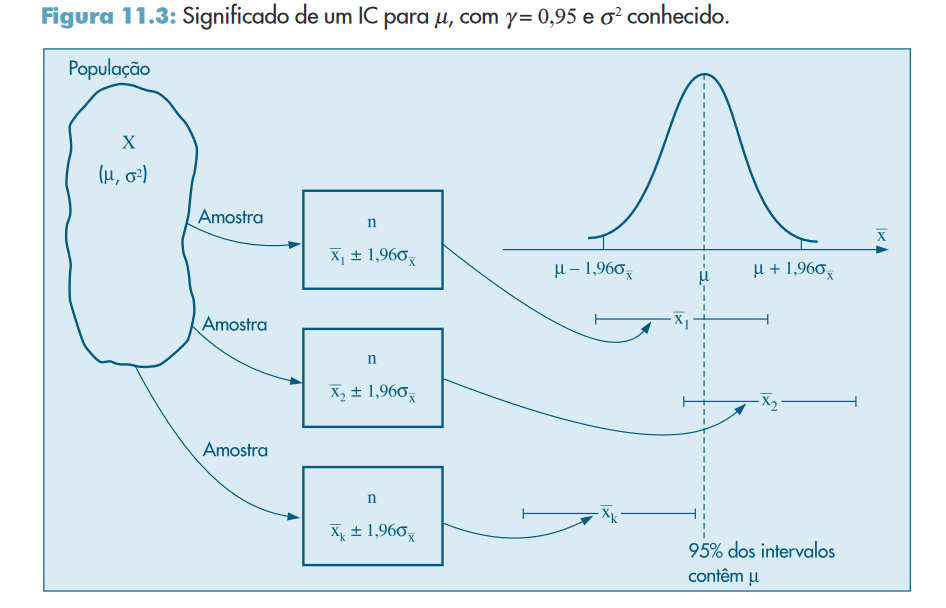
\includegraphics[scale=.5]{Figures/confidence-interval.PNG}
\end{figure}

\subsection{Bootstrapping}
Método de reamostragem que trata uma amostra como uma população finita; então são geradas amostras a partir da original, para estimar característica populacionais e fazer infêrencia sobre a população.

É uma classe de métodos de Monte Carlo não paramétricos que estimam a distribuição da população por reamostragem.

O termo “bootstrap” pode ser dirigido a bootstrap não-paramétrico ou bootstrap
paramétrico. Seguiremos com o primeiro.

A distribuição da população finita representada pela amostra pode ser encarada como uma pseudo-população, com características análogas às da verdadeira população. Através da geração repetida de amostras aleatórias, com reposição, desta pseudo-população (reamostragem), a distribuição de amostragem de uma estatística pode ser estimada. 

O bootstrap gera amostras aleatoriamente a partir da distribuição empírica da amostra.

Propriedades de um estimador tal como o viés ou o erro padrão podem ser estimadas
por reamostragem.


É possível utilizar bootstrapping para calcular um intervalo de confiança para avaliar a acurácia de um modelo em um conjunto de dados de teste. Inclusive, para estudar AUCROC.

Em séries temporais, é possível simular um conjunto de simulações, por boostrap, para cada tempo discreto no futuro e criar bandas com 95\% de probabilidade (empíricas) e assumir a média em cada tempo como sendo a predição.

\subsection{Methods of Evaluating Estimators}

\begin{itemize}
    \item \textbf{Standard Error (Erro Padrão)}: According to Bussab, if $\hat{\theta}$ is a estimator for $\theta$, we call the standard error (erro padrão) of $\hat{\theta}$ the following quantity:
    
    \begin{equation}
        EP(\hat{\theta}) = \sqrt{Var(\hat{\theta})}
    \end{equation}
    
    The variance of $\hat{\theta}$ depends of distribution parameters. Generally, to obtain an estimate of the standard error, we use:
    
    \begin{equation}
        \hat{EP(\hat{\theta})} = \sqrt{\hat{Var(\hat{\theta})}}
    \end{equation}
    
    The standard error for the mean $\bar{X}$ of a sample of size $n$ is $\sqrt{Var(X)/n}$
    
    \item \textbf{Mean Square Error (MSE) of an Estimator:} the mean square error (MSE) of an estimator $\hat{\theta}$ of a parameter $\theta$ is $E[(\hat{\theta} - \theta)^2]$. Do not confuse the MSE with the RMSE used to evaluate the predictions of a regression model.

\end{itemize}

\subsection{Fisher Information:} in mathematical statistics, the Fisher information (sometimes simply called information) is a way of measuring the amount of information that an observable random variable X carries about an unknown parameter $\theta$ of a distribution that models X.
    
    \begin{equation}
        \mathcal {I}(\theta )=\operatorname {E} \left[\left.\left({\frac {\partial }{\partial \theta }}\log f(X;\theta )\right)^{2}\right|\theta \right]=-\operatorname {E} \left[\left.\left({\frac {\partial^2 }{\partial \theta^2 }}\log f(X;\theta )\right)\right|\theta \right]=\int _{\mathbb {R} }\left({\frac {\partial }{\partial \theta }}\log f(x;\theta )\right)^{2}f(x;\theta )\,dx,
    \end{equation}
    
\subsection{Hessian Matrix:} Suppose $f:\mathbb{R}^n \to \mathbb{R}$ is a function taking as input a vector $\bold{x} \in \mathbb{R}^n$ and outputting a scalar $f(\bold{x}) \in \mathbb{R}$. If all second partial derivatives of $f$ exist, then the Hessian matrix $\bold{H}$ of $f$ is a square $n \times n$, usually defined and arranged as follows:
    
    \begin{equation}
        \mathbf {H} _{f}={\begin{bmatrix}{\dfrac {\partial ^{2}f}{\partial x_{1}^{2}}}&{\dfrac {\partial ^{2}f}{\partial x_{1}\,\partial x_{2}}}&\cdots &{\dfrac {\partial ^{2}f}{\partial x_{1}\,\partial x_{n}}}\\[2.2ex]{\dfrac {\partial ^{2}f}{\partial x_{2}\,\partial x_{1}}}&{\dfrac {\partial ^{2}f}{\partial x_{2}^{2}}}&\cdots &{\dfrac {\partial ^{2}f}{\partial x_{2}\,\partial x_{n}}}\\[2.2ex]\vdots &\vdots &\ddots &\vdots \\[2.2ex]{\dfrac {\partial ^{2}f}{\partial x_{n}\,\partial x_{1}}}&{\dfrac {\partial ^{2}f}{\partial x_{n}\,\partial x_{2}}}&\cdots &{\dfrac {\partial ^{2}f}{\partial x_{n}^{2}}}\end{bmatrix}}
    \end{equation}
\end{itemize} 
%% Chapter Template

\chapter{Python versus R} % Main chapter title

\label{ChapterX} % Change X to a consecutive number; for referencing this chapter elsewhere, use \ref{ChapterX}

%----------------------------------------------------------------------------------------
%	SECTION 1
%----------------------------------------------------------------------------------------

\section{Observações}

Python, currently, does not have libraries that perform the forward, backward and stepwise feature selection based on statistical methods (p-values). R does have pretty good libraries to work with that. 

%----------------------------------------------------------------------------------------
%	THESIS CONTENT - APPENDICES
%----------------------------------------------------------------------------------------

\appendix % Cue to tell LaTeX that the following "chapters" are Appendices

% Include the appendices of the thesis as separate files from the Appendices folder
% Uncomment the lines as you write the Appendices

%% Appendix A

\chapter{Frequently Asked Questions} % Main appendix title

\label{AppendixA} % For referencing this appendix elsewhere, use \ref{AppendixA}

\section{How do I change the colors of links?}

The color of links can be changed to your liking using:

{\small\verb!\hypersetup{urlcolor=red}!}, or

{\small\verb!\hypersetup{citecolor=green}!}, or

{\small\verb!\hypersetup{allcolor=blue}!}.

\noindent If you want to completely hide the links, you can use:

{\small\verb!\hypersetup{allcolors=.}!}, or even better: 

{\small\verb!\hypersetup{hidelinks}!}.

\noindent If you want to have obvious links in the PDF but not the printed text, use:

{\small\verb!\hypersetup{colorlinks=false}!}.

%\include{Appendices/AppendixB}
%\include{Appendices/AppendixC}

%----------------------------------------------------------------------------------------
%	BIBLIOGRAPHY
%----------------------------------------------------------------------------------------

\printbibliography[heading=bibintoc]

%----------------------------------------------------------------------------------------

\end{document}  
